\documentclass{article}
\usepackage{tikz}
\begin{document}
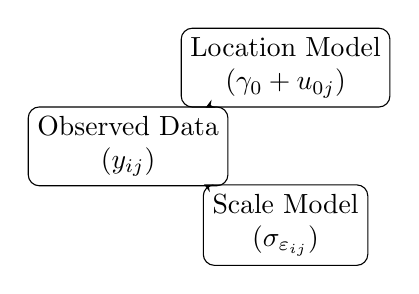
\begin{tikzpicture}[
    node distance=2cm,
    every node/.style={draw, align=center, rounded corners},
    ->, >=stealth
]
    \node (data) {Observed Data \\ (\(y_{ij}\))};
    \node (loc) [right of=data, yshift=1cm] {Location Model\\(\( \gamma_0 + u_{0j} \))};
    \node (scale) [right of=data, yshift=-1cm] {Scale Model\\(\( \sigma_{\varepsilon_{ij}} \))};

    \draw [->] (data) -- (loc);
    \draw [->] (data) -- (scale);
\end{tikzpicture}
\end{document}
